%%%%%%%%%%%%%%%%%%%%%%%%%%%%%%%%%%%%%%%%%%%%%%%%%%%%%%%%%%%%%%%%%%%%%%%%%%%%%%%%
% DUET ICRA 2026 draft.
% Based on the official Papercept ieeeconf template downloaded from:
% https://ras.papercept.net/conferences/support/files/ieeeconf.zip
%%%%%%%%%%%%%%%%%%%%%%%%%%%%%%%%%%%%%%%%%%%%%%%%%%%%%%%%%%%%%%%%%%%%%%%%%%%%%%%%

\documentclass[letterpaper, 10 pt, conference]{ieeeconf}

\IEEEoverridecommandlockouts
\overrideIEEEmargins

\usepackage{amsmath}
\usepackage{amssymb}
\usepackage{booktabs}
\usepackage{graphicx}
\usepackage{multirow}
\usepackage[table]{xcolor}
\usepackage{url}
\usepackage{balance}

\title{\LARGE \bf
DUET: Endogenous Failure Detection and Recovery via Dual-Action Manifold Alignment
}

\author{Anonymous Authors% <-this % stops a space
\thanks{This paper is an ICRA 2026 draft. Author names and affiliations are omitted for anonymous review.}
}

\begin{document}

\maketitle
\thispagestyle{empty}
\pagestyle{empty}

\begin{abstract}
Vision-language-action (VLA) models map vision and language to robot actions. With limited post-training demonstrations, however, they often cannot detect or recover from execution failures that move the robot out of distribution (OOD), such as mis-grasps, dropped objects, unexpected occlusions, and object or robot displacement. Many existing solutions rely on external failure detectors or costly intervention and recovery data, leaving detection loosely coupled with control. We introduce DUET (Dual-manifold Unified Execution and Transfer), a dual-action-head module that predicts relative and absolute actions. DUET uses the endogenous disagreement between the two heads as its primary failure signal, complemented by state-distribution distance. The absolute head excludes the current robot state and predicts RVQ-anchored global waypoints from vision and language, providing stable recovery targets when relative control becomes unreliable. We evaluate DUET on four LIBERO suites under five families of execution failures, and transfer the identical module to a $\pi_0$ backbone on a real Franka arm. DUET preserves nominal success ($96.9\%$ vs.\ $93.8\%$ for the relative-only baseline) while raising success under action-execution failures from $27.9\%$ to $64.6\%$ ($+36.7$ pp). Under our matched protocol, its disagreement score achieves the highest AUROC ($0.845$) among the evaluated success-only detectors. On hardware, DUET matches $\pi_0$ under nominal execution ($90.0\%$) and raises robot-state OOD success from $10.0\%$ to $77.5\%$.
\end{abstract}

\begin{figure*}[t]
\centering
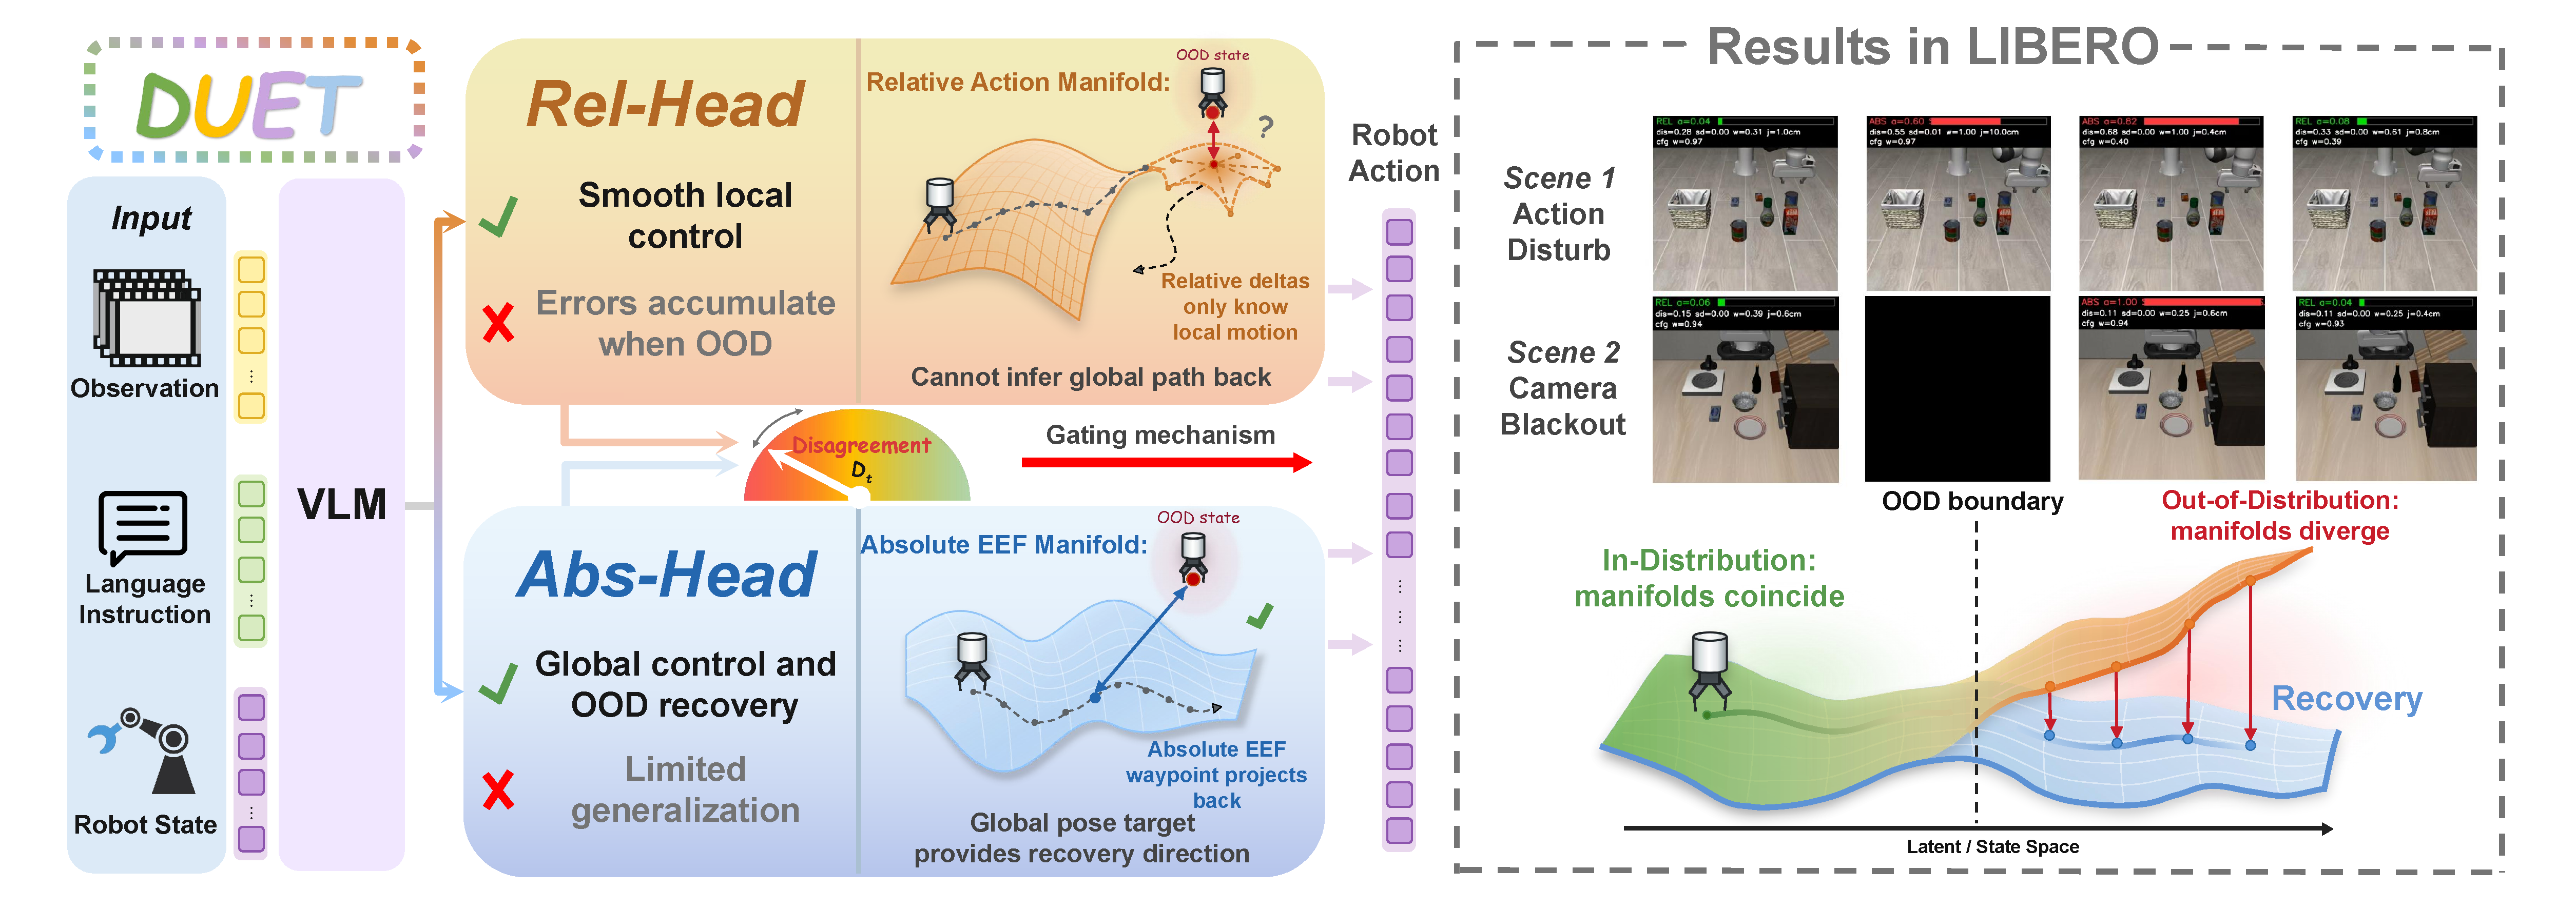
\includegraphics[width=0.96\textwidth]{figures/fig1.pdf}
\caption{Dual-manifold failure detection and recovery. The relative and absolute end-effector manifolds agree during nominal execution but diverge when a failure drives the system OOD, exposing an endogenous disagreement score $D_t$. Relative actions provide precise local motion, whereas absolute waypoints project execution toward a stable demonstrated-manifold anchor.}
\label{fig:teaser}
\end{figure*}

\section{INTRODUCTION}

Vision-language-action (VLA) policies adapt pretrained vision-language models to map visual observations and language instructions directly to robot actions \cite{openvla,starvla}. Despite their semantic generalization, policies post-trained on limited robot demonstrations remain vulnerable to failures during closed-loop execution. We focus on failures that drive the visual observation, robot--object configuration, or induced trajectory out of distribution (OOD) relative to successful demonstrations. They include policy-induced errors, such as an off-center grasp or an accidentally dropped object, as well as external events, such as transient occlusion or unexpected displacement of an object or the robot arm. After such events, a VLA may continue to produce locally plausible actions even though its trajectory is no longer supported by the demonstrations. Detecting these failures and actively recovering from them can therefore substantially improve task success and deployment reliability.

Existing approaches commonly introduce an external monitor, critic, verifier, or predictive model for failure detection \cite{faildetect}, and rely on large amounts of human takeover data collected during failed executions to learn recovery \cite{dagger,sirius,intervengen}. This process is costly because operators must continuously monitor rollouts and provide corrective actions across diverse visual, object, and robot-state failures. Moreover, detection and recovery are learned separately, so a failure alarm is not necessarily aligned with the action needed to recover. We instead seek a single policy that uses endogenous action information to detect and recover from OOD failures without additional failure or intervention data.

DUET takes disagreement between different action spaces as an endogenous signal for failure detection, as illustrated in Fig.~\ref{fig:teaser}. In our preliminary experiments, policies trained with relative actions produced smoother and more stable motions during nominal execution, but struggled to recover once a grasp or motion deviated because state-relative commands provide no explicit return target. In contrast, policies trained with absolute actions could redirect the robot toward trajectories supported by the demonstration distribution and retry after a failure. This complementary behavior motivates DUET to learn the same demonstrated behavior with a relative action head and an absolute action head. The relative head serves as the nominal controller, while the absolute head provides global recovery anchors. The two action spaces agree under in-domain execution but often diverge under the execution shifts considered here, thereby coupling failure detection and recovery through the same pair of predictions.

At inference time, DUET converts the predicted absolute waypoint into a correction from the live pose and compares it with the relative action. The two predictions remain consistent along successful trajectories but diverge when a failure drives execution OOD. Their disagreement, together with distance from the training state distribution, determines a soft fusion weight: DUET follows the smooth relative controller during nominal execution, shifts toward the absolute recovery target after failure, and returns to relative control after re-entering the demonstrated support. The same cross-space signal therefore both detects failure and determines the recovery direction, except when the observation itself is invalid and a cached waypoint must be held.

Our contributions are threefold:
\begin{itemize}
    \item We propose DUET, a dual-action-head VLA that learns relative and absolute action spaces from successful demonstrations and uses their endogenous disagreement to detect OOD-induced failures without an external detector.
    \item We design a stateless, RVQ-anchored absolute action head and an adaptive closed-loop controller that converts cross-space disagreement into stable recovery while preserving precise relative control under nominal conditions.
    \item We validate DUET on four LIBERO suites under five failure families---action-execution drift, robot displacement, grasp loss, transient occlusion, and external contact---and transfer the same module to a $\pi_0$ backbone on a real Franka arm.
\end{itemize}

\section{RELATED WORK}

\subsection{Runtime Failure Detection}
Runtime monitors score deviations through action consistency, representation novelty, likelihood, or task progress \cite{sentinel,faildetect,fiper,vlafail,rewindil}. Foundation-model detectors instead learn semantic failure scores or diagnoses, often from failed rollouts \cite{safe,aha}. These methods produce auxiliary alarms, diagnoses, or checkpoint lookups. DUET learns two action representations from successful demonstrations; the transported absolute prediction both creates the disagreement score and supplies an executable correction.

VLA-specific methods use internal features or external foundation models. SAFE learns a detector from successful and failed rollouts \cite{safe}, whereas AHA trains a VLM to detect and diagnose failures \cite{aha}. Such methods require additional supervision or a separate detector whose output is not a recovery action. DUET instead detects failures through disagreement between two action spaces learned within the policy, using OOD manifold inconsistency as both an alarm and a recovery signal.

\subsection{Recovery from Execution Failures}
Recovery methods commonly expand the training distribution with expert corrections. DAgger queries experts on policy-induced states \cite{dagger}; intervention-based methods collect human takeovers \cite{eil,sirius}; and IntervenGen transforms limited interventions into corrective trajectories \cite{intervengen}. These approaches reduce compounding errors but still require additional recovery actions.

Foundation-model systems instead use semantic supervisors. RACER learns from language-annotated recovery trajectories \cite{racer}, while AHA and VLM controllers diagnose failures and guide downstream correction \cite{aha,vlmrecovery}. Their detection and recovery components remain separately trained or prompted. DUET couples both capabilities without extra recovery data: absolute states from successful demonstrations provide recovery anchors, while cross-space disagreement determines when and how strongly to move toward them.

\section{METHOD}

\subsection{Problem Formulation}
At time $t$, the robot observes multi-view images $o_t$, a language instruction $l$, and proprioceptive state $s_t$. Trained only on successful demonstrations, DUET predicts the same behavior in two action representations over a horizon $K$:
\begin{align}
    \hat{\Delta A}_t &= f_{\mathrm{rel}}(o_t,l,s_t)
    \in \mathbb{R}^{K\times 7}, \\
    \hat{W}_t &= f_{\mathrm{abs}}(o_t,l)
    \in \mathbb{R}^{K\times 7}.
\end{align}
$\Delta A_t$ contains relative operational-space commands and $W_t$ absolute waypoints $[x,y,z,r_x,r_y,r_z,g]$. Recorded deltas and future end-effector states supervise the respective heads. Fusion acts on the 6-D pose component $a_p$; the deployed gripper command comes from the relative head.

\begin{figure}[!t]
\centering
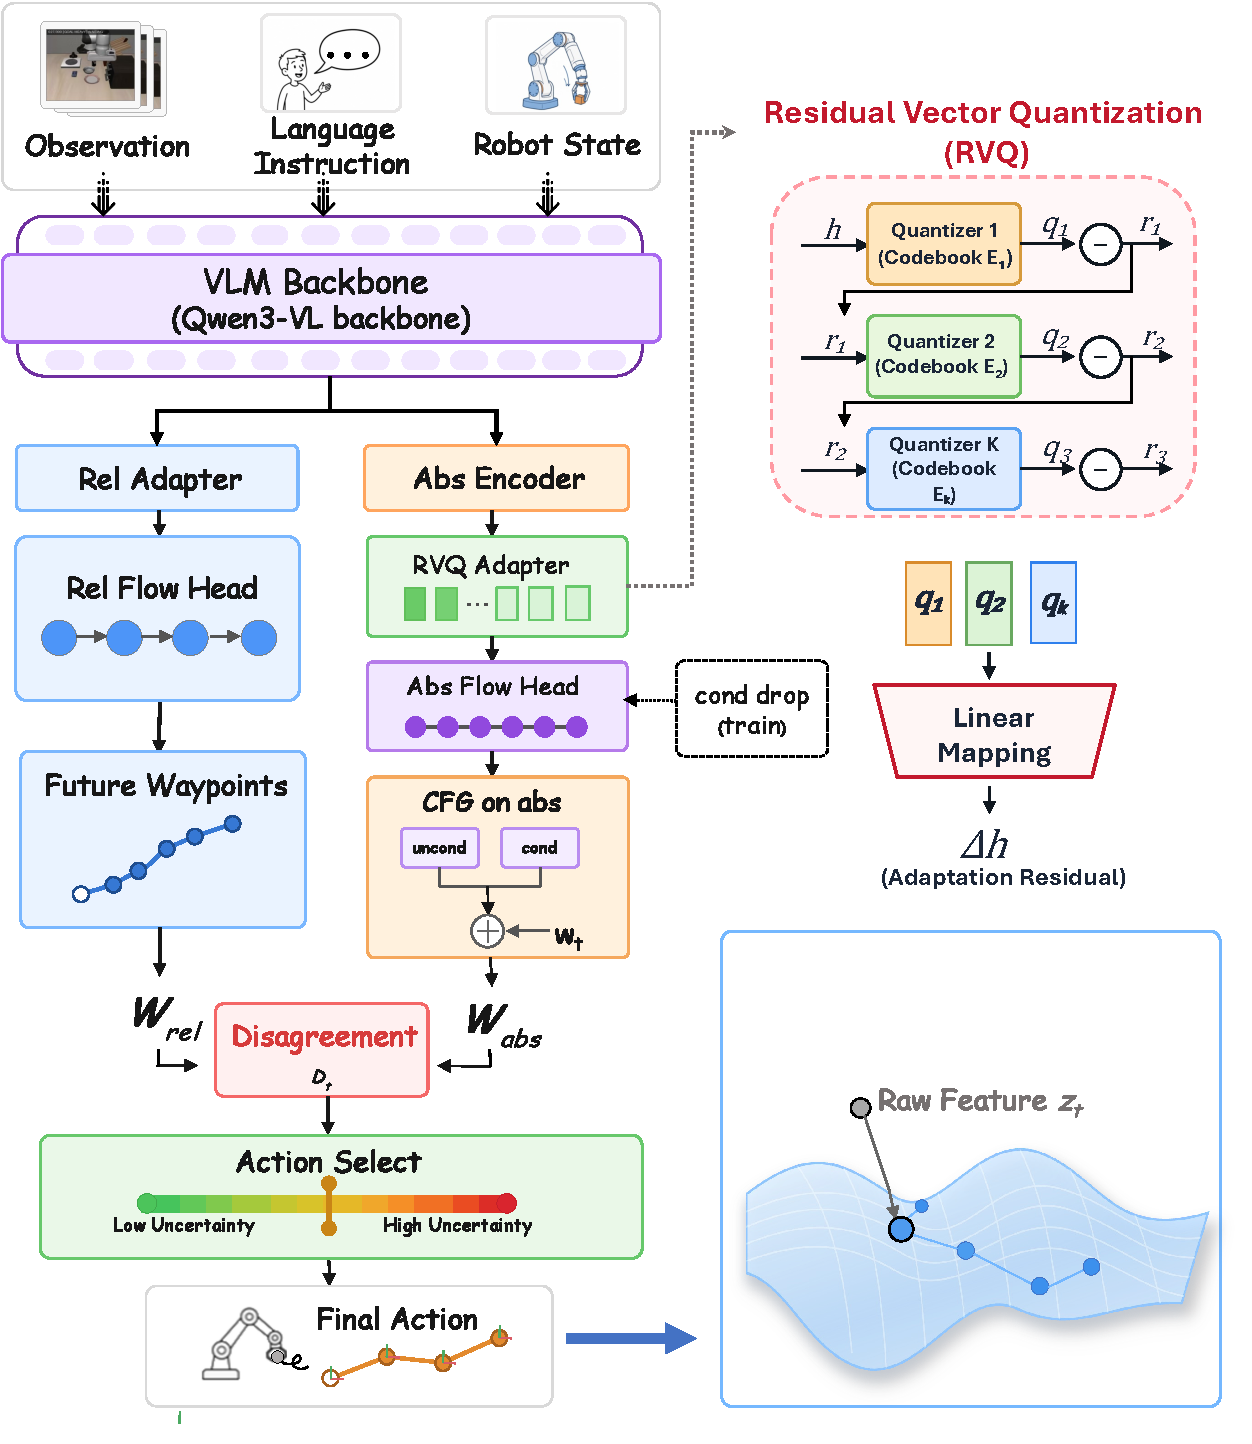
\includegraphics[width=\columnwidth]{figures/fig2.pdf}
\caption{DUET comprises a shared vision-language encoder, relative and absolute action heads, cross-space failure detection, and closed-loop recovery. Disagreement between state-aware relative control and RVQ-anchored absolute waypoints gates the switch from nominal execution to recovery.}
\label{fig:architecture}
\end{figure}

\subsection{Two Views of One Behavior}
\label{sec:manifolds}
We use geometry as intuition, not as a formal guarantee. For instruction $l$, successful end-effector poses occupy a demonstrated support $\mathcal{M}_l\subset SE(3)$. The relative head answers \emph{how to move next} from live pose $p_t$,
\begin{equation}
    \hat{\delta a}_{p,t} = f_{\mathrm{rel}}(o_t,l,s_t)_p,
\end{equation}
which is locally precise but provides no return destination off support. The absolute head answers \emph{where to be},
\begin{equation}
    \hat{w}_{p,t}=f_{\mathrm{abs}}(o_t,l)_p,
\end{equation}
providing a coarser target anchored by successful demonstrations.

We map the waypoint to a one-step correction at the live pose,
\begin{equation}
    c_t=\Psi_{p_t}(\hat{w}_{p,t}),
    \label{eq:transport_map}
\end{equation}
instantiated in Eq.~\eqref{eq:recovery_vector} by normalized translation and geodesic rotation residuals. This is a clipped first-order surrogate, not parallel transport on $SE(3)$.

On support, $c_t$ and $\hat{\delta a}_{p,t}$ describe the same behavior and should broadly agree. Off support, local extrapolation can diverge from the demonstrated anchor. We use their residual as a heuristic---not calibrated---failure score and $c_t$ as its implied recovery direction. Disagreement is neither necessary nor sufficient for failure: corrupted observations can degrade both heads together, as handled in Sec.~\ref{sec:method-gate}. We therefore validate it empirically in Sec.~\ref{sec:detection}.

\subsection{Dual-Head Architecture}
Figure~\ref{fig:architecture} shows the shared VLM and two flow-matching heads \cite{diffusionpolicy,pi0}. The relative head attends to the full sequence and receives $s_t$. The absolute head excludes state tokens from pooling, preserving a complementary observation-conditioned reference rather than a second state-conditioned local controller.

It pools its state-free hidden sequence $H^0$ and applies residual vector quantization (RVQ) \cite{vqvae,rvq}:
\begin{equation}
    Z_q=\operatorname{RVQ}\!\left(\operatorname{Pool}(H^0)\right).
\end{equation}
RVQ maps conditions to a discrete atlas of successful demonstrations. Its residual norm is auxiliary telemetry. Classifier-free guidance (CFG) \cite{cfg} softens recovery predictions toward the demonstrated waypoint marginal.

\subsection{Disagreement-Preserving Learning}
\label{sec:learning}
Both heads train on paired labels from every successful trajectory, with flow-matching objectives and an RVQ commitment loss:
\begin{equation}
    \mathcal{L} =
    \lambda_{\mathrm{rel}}\mathcal{L}_{\mathrm{rel}}
    + \lambda_{\mathrm{abs}}\mathcal{L}_{\mathrm{abs}}
    + \lambda_{\mathrm{vq}}\mathcal{L}_{\mathrm{vq}},
\label{eq:training_loss}
\end{equation}
where absolute labels are normalized future states and relative labels are recorded deltas. We omit cross-head consistency loss to preserve useful disagreement.

Asymmetric visual augmentation specializes the branches. The absolute head and RVQ adapter train on clean and perturbed observations so the global anchor remains stable under degraded input. The relative head is optimized only on the clean subset $\mathcal{B}_{\mathrm{clean}}$:
\begin{equation}
    \mathcal{L}_{\mathrm{rel}} =
    \frac{1}{|\mathcal{B}_{\mathrm{clean}}|}
    \sum_{i \in \mathcal{B}_{\mathrm{clean}}}
    \ell_{\mathrm{FM}}(\hat{\Delta a}^{(i)}, \Delta a^{(i)}).
\end{equation}
This keeps the relative head sensitive and the absolute branch robust. For CFG, the absolute head uses learned null tokens on a subset of samples.

\subsection{Joint Failure Detection and Recovery}
\label{sec:method-gate}
At deployment the policy returns both unnormalized action chunks. With live pose $p_t=(x_t,R_t)$ and absolute waypoint $\hat{w}_{p,t}=(\hat{x}_t,\hat{R}_t)$, the transport map in Eq.~\eqref{eq:transport_map} is
\begin{equation}
    c_t=\operatorname{clip}\!\left(
    \begin{bmatrix}
    (\hat{x}_t-x_t)/\sigma_p \\
    \operatorname{Log}(\hat{R}_tR_t^{-1})/\sigma_R
    \end{bmatrix},-1,1\right),
    \label{eq:recovery_vector}
\end{equation}
where $\operatorname{Log}:SO(3)\rightarrow\mathfrak{so}(3)$ is the geodesic rotation correction and $\sigma_p,\sigma_R$ convert pose error into action units. Cross-space disagreement is the primary failure signal,
\begin{equation}
    D_t=\frac{\left\|c_t-
    \operatorname{clip}(\hat{\delta a}_{p,t},-1,1)\right\|_2}{\sqrt{6}}.
    \label{eq:disagreement}
\end{equation}
A coarse state-distance term measures normalized violation of the training-state bounds:
\begin{equation}
    S_t =
    \mathrm{mean}\left[
    \frac{\max(s_{\min} - p_t, 0)}{s_{\max}-s_{\min}}
    +
    \frac{\max(p_t - s_{\max}, 0)}{s_{\max}-s_{\min}}
    \right].
\end{equation}
The failure score and recovery weight are $q_t = D_t + \lambda S_t$ and $\alpha_t = \sigma(k(q_t-\tau))$. DUET interpolates local execution and global recovery while keeping relative gripper control:
\begin{align}
    a_t &= [a_{p,t},a_{g,t}], \\
    a_{p,t} &= (1-\alpha_t)\hat{\delta a}_{p,t} + \alpha_t c_t, \\
    a_{g,t} &= \hat{\delta a}_{g,t},
    \label{eq:fused_action}
\end{align}
Relative control dominates on support; rising $q_t$ shifts the pose command toward $c_t$, and control returns after realignment. The previous fusion weight also sets the next absolute-head CFG scale, $w_t = w_{\max}-(w_{\max}-w_{\min})\alpha_{t-1}$. Thus $D_t$ determines \emph{when} and $c_t$ \emph{how} to recover. If vision is invalid, a guard freezes the last reliable waypoint and holds $\alpha_t{=}1$ until it returns.

\section{EXPERIMENTS}
\label{sec:experiments}

\begin{samepage}
We organize the simulation experiments around three questions:
\begin{itemize}
    \setlength{\itemsep}{0pt}
    \setlength{\parsep}{0pt}
    \setlength{\topsep}{2pt}
    \item[\textbf{(Q1)}] \textbf{Failure-aware retry:} Can DUET convert execution failures into successful task completion?
    \item[\textbf{(Q2)}] \textbf{Baseline comparison:} Does DUET improve robustness without sacrificing nominal performance?
    \item[\textbf{(Q3)}] \textbf{Endogenous OOD detection:} Can cross-space disagreement detect failures using only successful demonstrations?
\end{itemize}
Closed-loop retry is the primary metric; nominal and detection results then isolate the source of that gain.
\end{samepage}

\subsection{Evaluation Protocol}
\label{sec:protocol}
We evaluate four LIBERO suites \cite{libero}, each with $10$ tasks and $50$ initial states per task, using suite-specific $10$k-step checkpoints trained only on successful demonstrations.

StarVLA \cite{starvla} is the external relative-action baseline. DUET-Rel ($\alpha_t{=}0$) and DUET share a checkpoint, so their difference isolates adaptive recovery, whereas StarVLA$\to$DUET-Rel captures dual-head co-training. Absolute-only ($\alpha_t{=}1$) and fixed fusion ($\alpha_t{=}0.5$) are inference-time ablations. DUET uses Qwen-VL features (size $2048$), 16-/8-layer relative/absolute DiT-B heads, and $16$ RVQ tokens from three codebooks (size $512$, dimension $256$), with $p_{\mathrm{aug}}{=}0.3$, $p_{\mathrm{drop}}{=}0.15$, $\lambda{=}1$, $\tau{=}0.5$, and $k{=}8$.

Perturbations use deterministic seeds and matched $(\mathrm{task},\mathrm{initial\ state})$ keys. Fixed steps place each disturbance in a meaningful phase: initial reach (action, step $5$), transport (teleport, $39$), after gripper closure (drop, $67$), and approach (blackout, $23$). This ensures identical interventions across methods but samples only one recovery horizon per family; later injection leaves less time to recover, as reflected by Spatial teleport. We retain episodes ending before injection, report coverage for semantic preconditions, and use paired McNemar tests. Table~\ref{tab:taxonomy} summarizes the families; external force is evaluated separately.

\begin{table}[t]
\caption{Execution-failure families and the quantity driven out of distribution.}
\label{tab:taxonomy}
\centering
\resizebox{\columnwidth}{!}{%
\begin{tabular}{lll}
\toprule
Family & Protocol & What becomes OOD \\
\midrule
Action execution & Action perturbation (step $5$) & Command-to-motion map \\
Robot displacement & EEF teleport (step $39$) & Robot-arm pose \\
Object / grasp & Vertical grasp drop (step $67$) & Robot--object configuration \\
Visual occlusion & Camera blackout (step $23$) & Current visual observation \\
Contact / scene & External force & Robot--world interaction \\
\bottomrule
\end{tabular}}
\end{table}

\begin{figure}[t]
\centering
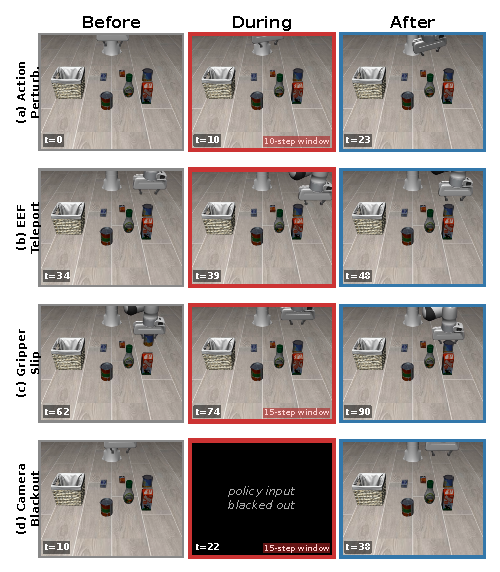
\includegraphics[width=\columnwidth]{figures/fig_perturbation_showcase.pdf}
\caption{Object-suite keyframes before, during, and after (a) action perturbation, (b) EEF teleport, (c) grasp drop, and (d) camera blackout.}
\label{fig:showcase}
\end{figure}

\subsection{\textbf{(Q1)} Failure-Aware Retry}
\label{sec:retry}
Table~\ref{tab:ood_detailed} reports closed-loop success. Against shared-checkpoint DUET-Rel, DUET improves action perturbation from $27.9\%$ to $64.6\%$, displacement from $34.5\%$ to $59.4\%$, grasp loss from $89.2\%$ to $95.2\%$, and occlusion from $73.5\%$ to $90.8\%$, exceeding StarVLA in every aggregate.

\begin{table*}[!t]
\caption{Closed-loop success (\%; $N{=}500$ per cell). Overall combines medium$+$severe across suites. Rel$\to$DUET has McNemar $p{<}10^{-3}$ except teleport/Spatial ($p{=}0.21/0.067$) and blackout/Object medium.}
\label{tab:ood_detailed}
\centering
\footnotesize
\begin{tabular*}{\textwidth}{@{\extracolsep{\fill}} l cccc @{\hspace{1.2em}} cccc @{}}
\toprule
& \multicolumn{4}{c}{Medium} & \multicolumn{4}{c}{Severe} \\
\cmidrule(lr){2-5}\cmidrule(l){6-9}
Suite & StarVLA & Rel. & DUET & $\Delta$ & StarVLA & Rel. & DUET & $\Delta$ \\
\midrule
\multicolumn{9}{@{}l}{\textit{(i) Action perturbation (step $5$)}} \\
Spatial    & 60.0 & 54.0 & 74.0 & $+20.0$ & 14.0 & 12.8 & 43.2 & $+30.4$ \\
Object     & 41.6 & 48.8 & 84.4 & $+35.6$ &  7.8 &  7.8 & 60.6 & $+52.8$ \\
Goal       & 52.2 & 47.2 & 74.2 & $+27.0$ & 18.8 & 10.6 & 52.6 & $+42.0$ \\
LIBERO-10  & 36.2 & 36.6 & 78.6 & $+42.0$ &  6.2 &  5.4 & 49.0 & $+43.6$ \\
\textbf{Overall} & 29.6 & \textbf{27.9} & \textbf{64.6} & $\mathbf{+36.7}$ & \multicolumn{4}{c}{\textit{med$+$sev combined}} \\
\midrule
\multicolumn{9}{@{}l}{\textit{(ii) EEF teleport (step $39$)}} \\
Spatial    & 55.4 & 54.6 & 57.6 & $+3.0$  & 46.8 & 48.2 & 52.6 & $+4.4$ \\
Object     & 43.4 & 36.2 & 76.0 & $+39.8$ & 21.2 & 20.8 & 68.4 & $+47.6$ \\
Goal       & 41.6 & 33.4 & 52.4 & $+19.0$ & 30.4 & 28.2 & 50.6 & $+22.4$ \\
LIBERO-10  & 40.4 & 35.8 & 60.8 & $+25.0$ & 21.4 & 18.4 & 56.8 & $+38.4$ \\
\textbf{Overall} & 37.6 & \textbf{34.5} & \textbf{59.4} & $\mathbf{+24.9}$ & \multicolumn{4}{c}{\textit{med$+$sev combined}} \\
\midrule
\multicolumn{9}{@{}l}{\textit{(iii) Vertical grasp drop (Object only, medium, step $67$)}} \\
Object     & 90.6 & 89.2 & \textbf{95.2} & $\mathbf{+6.0}$  & \multicolumn{4}{c}{---} \\
\midrule
\multicolumn{9}{@{}l}{\textit{(iv) Camera blackout (step $23$)}} \\
Spatial    & 81.0 & 88.0 & 94.4 & $+6.4$  & 42.4 & 63.2 & 95.2 & $+32.0$ \\
Object     & 91.8 & 98.6 & 96.8 & $-1.8$  & 64.2 & 95.0 & 97.2 & $+2.2$ \\
Goal       & 65.4 & 86.0 & 86.4 & $+0.4$  & 35.4 & 65.8 & 85.8 & $+20.0$ \\
LIBERO-10  & 60.0 & 65.6 & 84.2 & $+18.6$ & 24.4 & 25.6 & 86.2 & $+60.6$ \\
\textbf{Overall} & 58.1 & \textbf{73.5} & \textbf{90.8} & $\mathbf{+17.3}$ & \multicolumn{4}{c}{\textit{med$+$sev combined}} \\
\bottomrule
\end{tabular*}
\end{table*}

\emph{Action and robot displacement.} The intact scene supplies a return target absent from relative control. DUET gains $36.7$ pp under action perturbation and $24.9$ pp under teleport. Spatial teleport is not significant ($p{=}0.21/0.067$), partly because some episodes finish before injection.

\emph{Grasp and vision.} A $5$\,cm drop yields a smaller but significant $6.0$ pp gain ($p{=}2.4{\times}10^{-5}$; coverage $\geq98.8\%$). During blackout, the validity guard rather than disagreement drives the $17.3$ pp gain; Object-medium is the sole nonsignificant regression ($-1.8$ pp).

\emph{Contact.} In $4{,}000$ external-force episodes, DUET reaches $95.95\%$ versus $92.22\%$, without suite-level regression.

\begin{figure}[t]
\centering
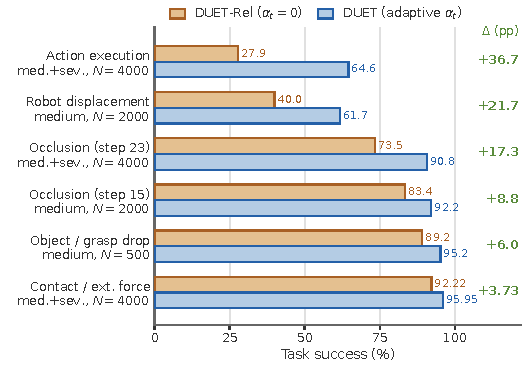
\includegraphics[width=\columnwidth]{figures/fig_ood_overall_success.pdf}
\caption{Paired DUET-Rel$\to$DUET success gain by family.}
\label{fig:overall}
\end{figure}

\paragraph{Mechanism evidence.}
Figure~\ref{fig:telemetry} shows switch-and-return: arm-state OOD raises $\alpha_t$ and activates correction; after realignment, relative control resumes. World-state responses are weaker, while complete visual dropout invokes the guard.

\begin{figure}[t]
\centering
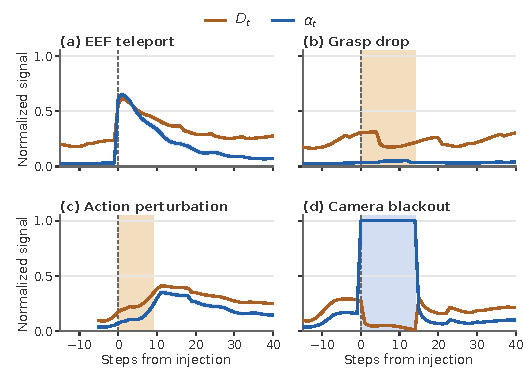
\includegraphics[width=\columnwidth]{figures/fig_ood_mechanism_grid.pdf}
\caption{$D_t$ and $\alpha_t$ on Object, aligned to injection (mean, pointwise 95\% CI): arm-state OOD (a,c), world-state change (b), and validity-guard override (d).}
\label{fig:telemetry}
\end{figure}

On Object teleport (Fig.~\ref{fig:manifold}; $n{=}484$--$498$), DUET closes $4.69$\,cm within $32$ steps and re-enters the clean-trajectory neighborhood in $97.9\%$ of episodes (median $16$ steps), versus $0.71$\,cm, $62.5\%$, and $58$ steps for DUET-Rel. Absolute-only reaches $99.6\%$ re-entry but zero task success, confirming that re-entry is a mechanism rather than the objective.

\begin{figure}[t]
\centering
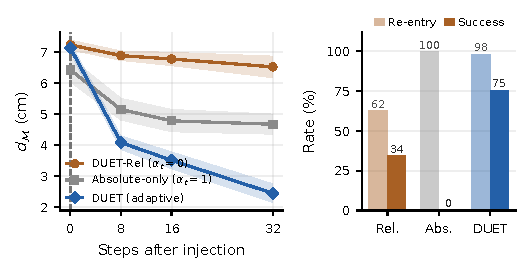
\includegraphics[width=\columnwidth]{figures/fig_manifold_distance.pdf}
\caption{Object EEF teleport (medium, step $39$; $n{=}484$--$498$). Left: distance to the clean-trajectory reference after injection. Right: re-entry and final task success.}
\label{fig:manifold}
\end{figure}

Together these results answer \textbf{Q1}: DUET converts recoverable deviations into successful retries, while grasp changes and invalid vision bound disagreement alone.

\subsection{\textbf{(Q2)} Baseline Comparison}
\label{sec:nominal}
Table~\ref{tab:nominal} compares nominal performance. Adaptive fusion raises the shared checkpoint from $93.8\%$ to $96.9\%$, matching the strongest reported average; the gap isolates fusion rather than capacity or training data.

\begin{table}[t]
\caption{Nominal LIBERO success (\%). Reported methods provide external context: StarVLA-GR00T uses joint $30$k training, whereas DUET uses suite-specific $10$k checkpoints.}
\label{tab:nominal}
\centering
\resizebox{\columnwidth}{!}{%
\begin{tabular}{lccccc}
\toprule
Method & Spatial & Object & Goal & LIBERO-10 & Avg. \\
\midrule
$\pi_{0.5}$ (reported) & 98.8 & 98.2 & 98.0 & 92.4 & 96.9 \\
StarVLA-GR00T (reported) & 97.8 & 98.8 & 97.4 & 92.0 & 96.5 \\
\midrule
DUET-Rel ($\alpha_t{=}0$) & 98.0 & 99.2 & 92.0 & 86.0 & 93.8 \\
\rowcolor{gray!20}
DUET & 98.8 & 99.4 & 97.6 & 91.8 & \textbf{96.9} \\
\bottomrule
\end{tabular}}
\end{table}

\subsection{\textbf{(Q3)} Endogenous OOD Detection}
\label{sec:detection}
Table~\ref{tab:detection} isolates the signal that triggers recovery, comparing $D_t$ with success-only detectors under matched protocols \cite{faildetect,sentinel}. Unlike these standalone scores, $D_t$ is coupled to the transported correction $c_t$.

\begin{table}[t]
\caption{Failure detection under matched protocols. All metrics are higher-is-better; bold denotes the best result in each column.}
\label{tab:detection}
\centering
\resizebox{\columnwidth}{!}{%
\begin{tabular}{@{}lcccc@{}}
\toprule
Method & TPR $\uparrow$ & TNR $\uparrow$ & AUROC $\uparrow$ & Loc.@16 $\uparrow$ \\
\midrule
logpZO \cite{faildetect} & 0.889 & 0.243 & 0.817 & \textbf{0.569} \\
RND \cite{rnd,faildetect} & 0.842 & \textbf{0.361} & 0.549 & 0.330 \\
PCA-kmeans \cite{faildetect} & 0.884 & 0.283 & 0.625 & 0.503 \\
STAC \cite{sentinel} & 0.839 & 0.311 & 0.494 & 0.260 \\
\rowcolor{gray!20}
DUET ($D_t$) & \textbf{0.900} & 0.265 & \textbf{0.845} & 0.523 \\
\bottomrule
\end{tabular}}
\end{table}

DUET leads AUROC ($0.845$) and TPR ($0.900$), but RND leads TNR and logpZO localization. All methods' low TNR ($0.24$--$0.36$) implies frequent nominal hard-threshold triggers. DUET instead uses a soft weight whose clean mean is $\alpha_t{=}0.139$, preserving nominal success; applications with costly false positives would require a stricter operating point. Thus disagreement offers the strongest ranking here and uniquely supplies the correction, but does not dominate every threshold metric.

\subsection{Ablations}
\label{sec:ablations}
Table~\ref{tab:main_results} isolates fusion. Absolute-only lacks local precision, while fixed fusion harms nominal execution and under-corrects disturbances; adaptive fusion succeeds in both regimes.

\begin{table}[t]
\caption{Fusion ablations, success (\%). Four-suite rows use $N{=}2000/2000/4000$; static gates use matched Object protocols ($N{=}500$).}
\label{tab:main_results}
\centering
\resizebox{\columnwidth}{!}{%
\begin{tabular}{llccc}
\toprule
Controller & Gate & Clean & Robot displ. & Action exec. \\
\midrule
\multicolumn{5}{@{}l}{\textit{Four-suite average}} \\
DUET-Rel & $\alpha_t{=}0$ & 93.8 & 40.0 & 27.9 \\
\rowcolor{gray!20}
DUET & adaptive $\alpha_t$ & \textbf{96.9} & \textbf{61.7} & \textbf{64.6} \\
\midrule
\multicolumn{5}{@{}l}{\textit{Object suite, matched protocol}} \\
DUET-Rel & $\alpha_t{=}0$ & 99.2 & 36.2 & 48.8 \\
Absolute-only & $\alpha_t{=}1$ & 5.2 & 1.1 & 0.8 \\
Fixed fusion & $\alpha_t{=}0.5$ & 46.2 & 39.4 & 41.0 \\
\rowcolor{gray!20}
DUET & adaptive $\alpha_t$ & 99.2 & \textbf{76.0} & \textbf{84.4} \\
\bottomrule
\end{tabular}}
\end{table}

Table~\ref{tab:ablations} isolates training choices. In this configuration, replacing RVQ with an MLP collapses the absolute branch; symmetric augmentation weakens specialization, and fixed CFG reduces OOD performance.

\begin{table}[t]
\caption{Component ablations, success (\%). CFG uses Object ($N{=}500$); retrains use LIBERO-10 ($N{=}500/500/1000$).}
\label{tab:ablations}
\centering
\resizebox{\columnwidth}{!}{%
\begin{tabular}{lccc}
\toprule
Variant & Clean & Robot displ. & Action exec. \\
\midrule
\multicolumn{4}{@{}l}{\textit{CFG schedule, Object suite}} \\
No adaptive CFG & 88.2 & 52.6 & 57.2 \\
\rowcolor{gray!20}
Full DUET & 99.2 & 76.0 & 84.4 \\
\midrule
\multicolumn{4}{@{}l}{\textit{Training replacements, LIBERO-10}} \\
RVQ $\rightarrow$ MLP & 0.0 & 0.0 & 0.0 \\
Symmetric augmentation & 86.8 & 58.6 & 60.9 \\
\rowcolor{gray!20}
Full DUET & 91.8 & 60.8 & 63.8 \\
\bottomrule
\end{tabular}}
\end{table}

\paragraph{Fusion on clean trajectories.}
Across $2{,}000$ clean episodes, mean $\alpha_t$ is $0.139$, its $95^{\mathrm{th}}$ percentile is $0.339$, and only $1.7\%$ of steps exceed $0.5$; relative control remains dominant.

\paragraph{Sensitivity to $\tau$ and $k$.}
Figure~\ref{fig:sensitivity} shows a broad Object region above $90\%$ nominal and $75\%$ OOD success; $\tau{=}0.5,k{=}8$ lies within it.

\begin{figure}[t]
\centering
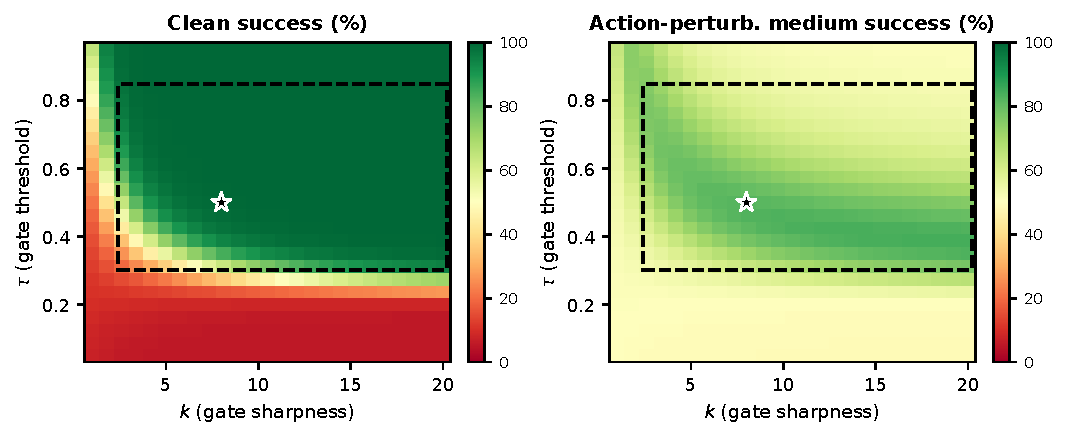
\includegraphics[width=\columnwidth]{figures/fig_sensitivity_heatmap.pdf}
\caption{Object sensitivity to $\tau,k$ from $500$ clean and $500$ perturbed traces. Rectangle: clean $>90\%$, OOD $>75\%$; star: operating point.}
\label{fig:sensitivity}
\end{figure}

\subsection{Real-Robot Evaluation}
\label{sec:real_robot}
We transfer the unchanged DUET module from StarVLA to $\pi_0$ (OpenPi) \cite{pi0}. A 7-DoF Franka Panda uses wrist and third-person cameras at $20$\,Hz. Each task is fine-tuned for $5$k steps from $\pi_0$-base on $50$ VR demonstrations. The four tasks are pick-and-place, pushing, drawer opening, and wiping (Fig.~\ref{fig:real_tasks}, left).

\begin{figure*}[t]
\centering
\begin{minipage}[c]{0.546\textwidth}
\centering
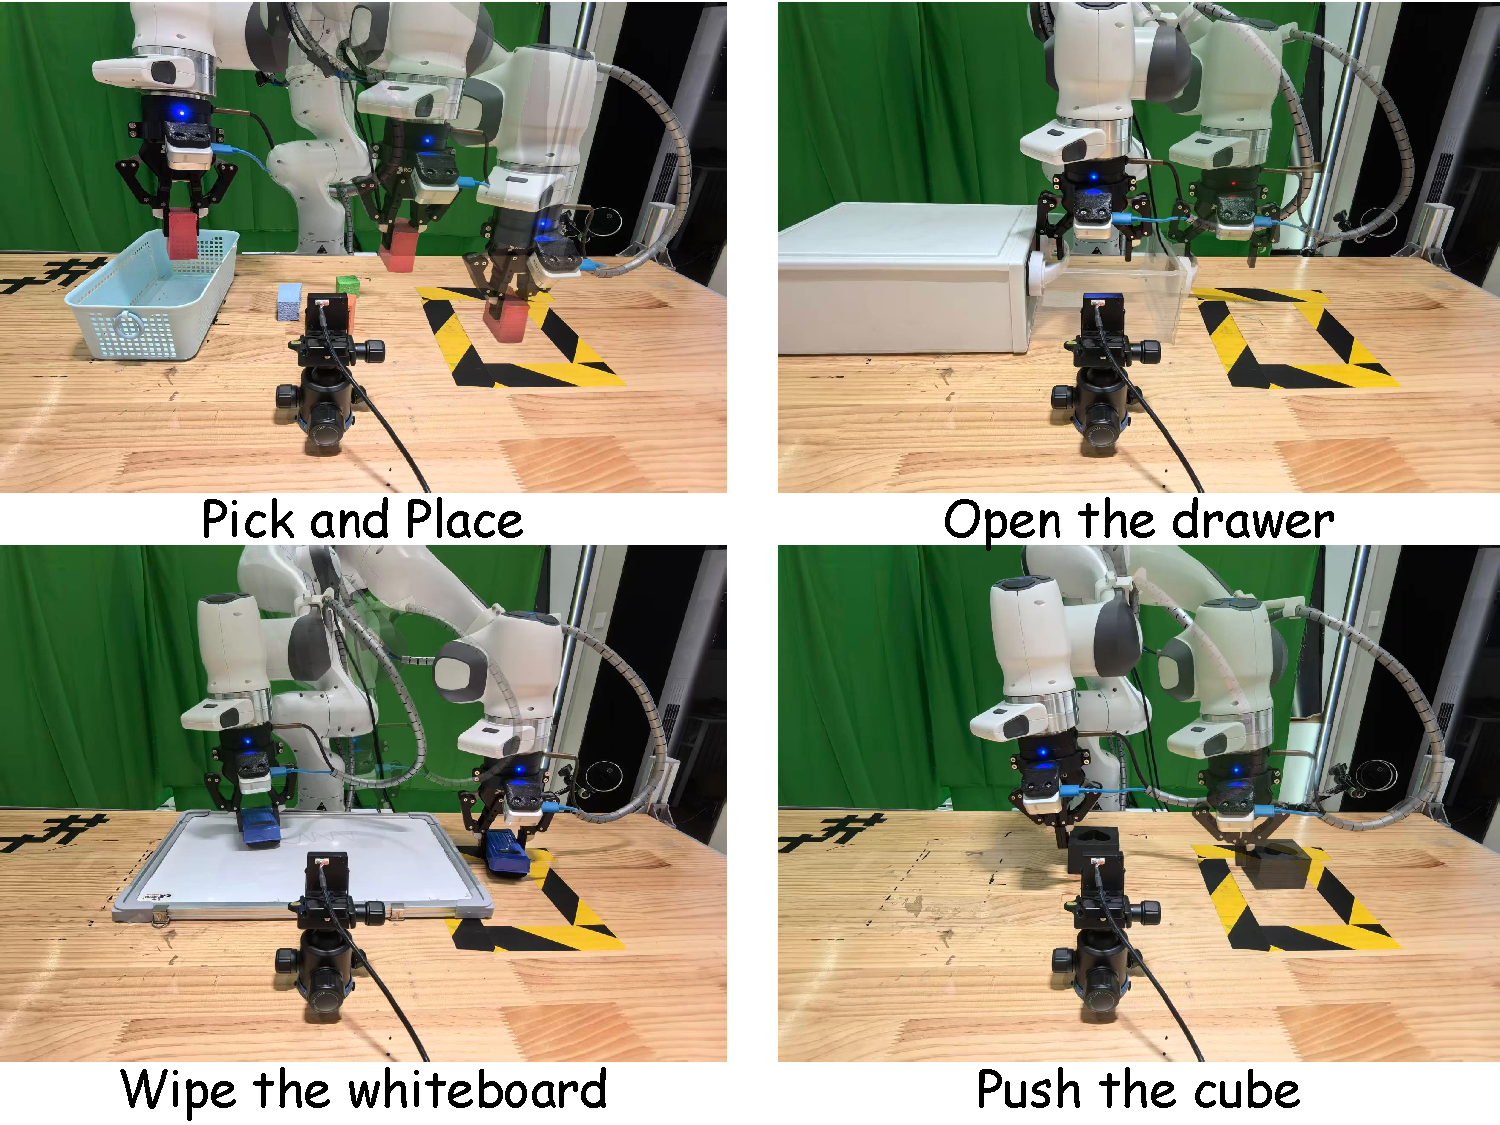
\includegraphics[width=\linewidth]{figures/real-robot-task.pdf}
\end{minipage}\hfill
\begin{minipage}[c]{0.434\textwidth}
\centering
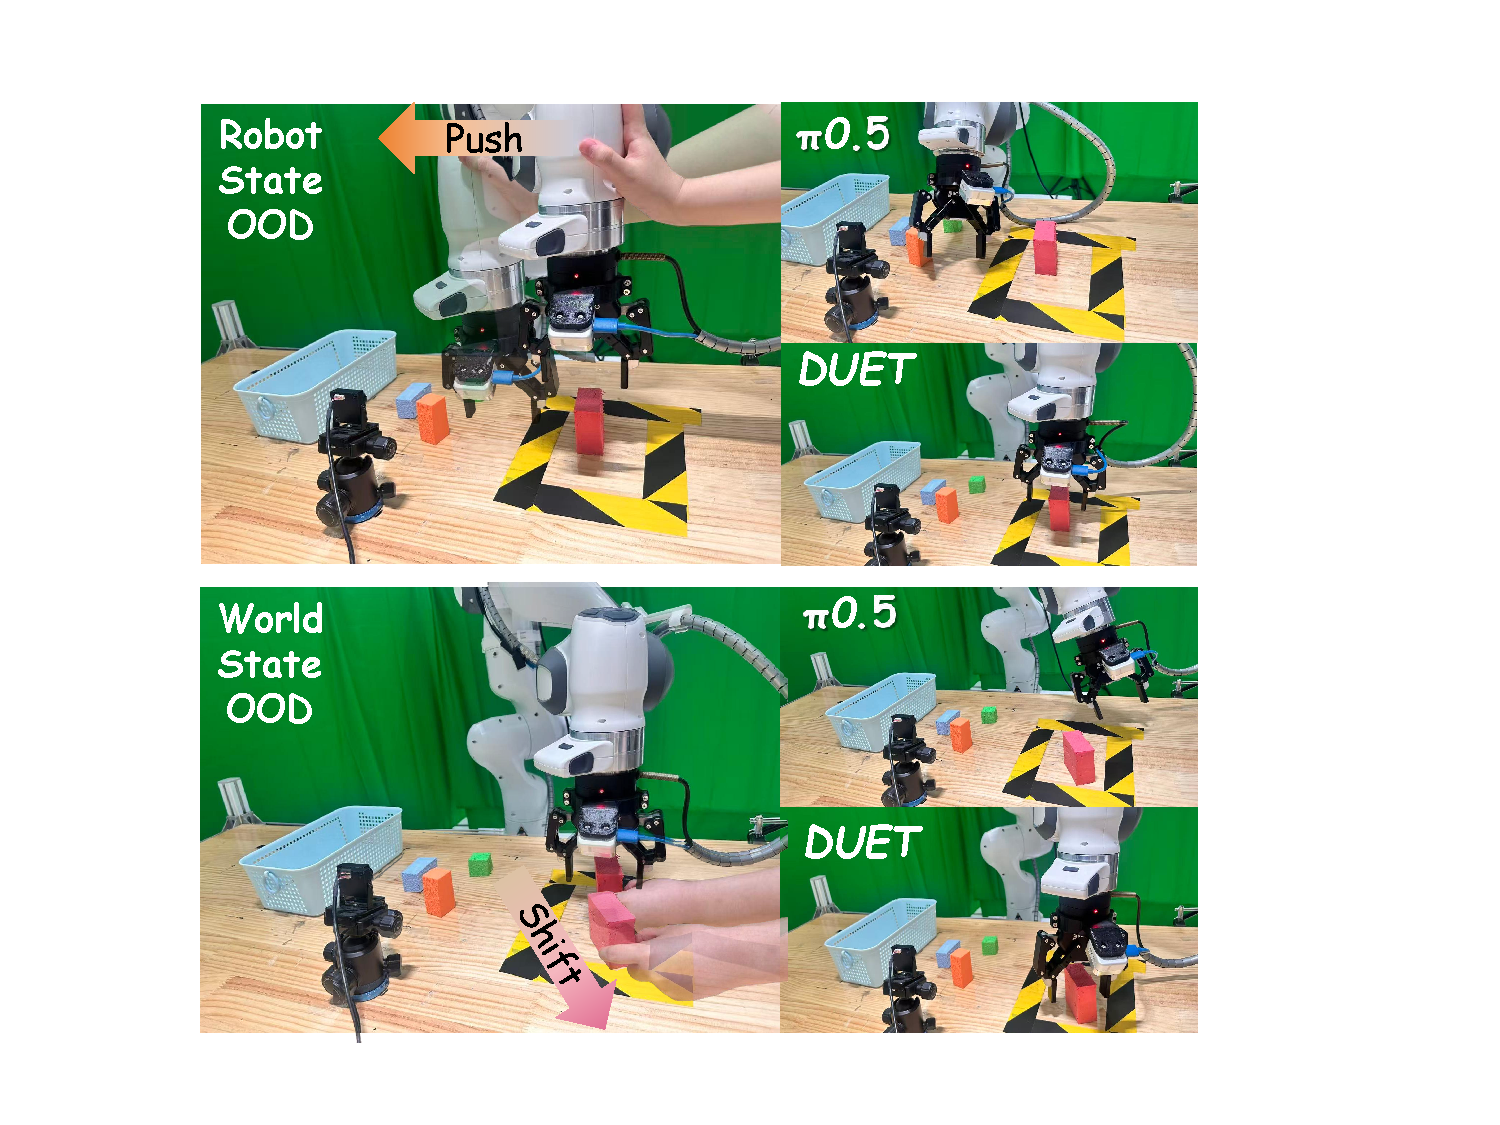
\includegraphics[width=\linewidth]{figures/oodrealbot.pdf}
\end{minipage}
\caption{Real-robot evaluation on a Franka Emika Panda. Left: four tasks (pick-and-place, drawer opening, whiteboard wiping, and block pushing). Right: qualitative recovery on block pushing. Top: robot-state EEF shift---$\pi_0$ fails, DUET recovers. Bottom: world-state cube shift---$\pi_0$ pushes empty space, DUET reacquires the object.}
\label{fig:real_tasks}
\label{fig:real_ood}
\end{figure*}

Each task is evaluated under nominal execution and two OOD families ($N{=}20$ trials per cell): a random-direction EEF shift (robot state) and an object displacement (world state), with task-specific intervention phases and magnitudes. Random directions are paired across $\pi_0$ and $\pi_0$+DUET.

\begin{table}[t]
\caption{Real-robot success (\%) with a $\pi_0$-base backbone ($N{=}20$ trials per cell; Overall pools $N{=}80$). Robot-state: random-direction EEF shift. World-state: object displacement. $\Delta$: $\pi_0$+DUET minus $\pi_0$.}
\label{tab:real_robot}
\centering
\footnotesize
\setlength{\tabcolsep}{2.6pt}
\resizebox{\columnwidth}{!}{%
\begin{tabular}{@{}l cc ccc ccc@{}}
\toprule
& \multicolumn{2}{c}{Nominal} & \multicolumn{3}{c}{Robot-state (EEF shift)} & \multicolumn{3}{c}{World-state (Obj.\ shift)} \\
\cmidrule(lr){2-3}\cmidrule(lr){4-6}\cmidrule(l){7-9}
Task & $\pi_0$ & +DUET & $\pi_0$ & +DUET & $\Delta$ & $\pi_0$ & +DUET & $\Delta$ \\
\midrule
Pick-and-place    & 95.0 & 95.0 & 15.0 & 85.0 & $+70.0$ &  5.0 & 50.0 & $+45.0$ \\
Block pushing     & 95.0 & 90.0 & 10.0 & 75.0 & $+65.0$ &  0.0 & 60.0 & $+60.0$ \\
Drawer opening    & 95.0 & 95.0 & 10.0 & 80.0 & $+70.0$ & 20.0 & 70.0 & $+50.0$ \\
Whiteboard wiping & 75.0 & 80.0 &  5.0 & 70.0 & $+65.0$ &  0.0 & 55.0 & $+55.0$ \\
\midrule
\rowcolor{gray!20}
\textbf{Overall}  & 90.0 & 90.0 & 10.0 & \textbf{77.5} & $\mathbf{+67.5}$ & 6.3 & \textbf{58.8} & $\mathbf{+52.5}$ \\
\bottomrule
\end{tabular}}
\end{table}

DUET preserves $\pi_0$'s $90.0\%$ nominal success (Table~\ref{tab:real_robot}). It raises robot-state OOD success from $10.0\%$ to $77.5\%$ and harder world-state OOD from $6.3\%$ to $58.8\%$. This transfers the same gate to hardware without a new detector or recovery dataset.

\section{LIMITATIONS}

DUET requires absolute-state labels aligned with relative chunks and may need hardware calibration. Its min--max state proxy can miss multimodal structure, while the stateless absolute branch can lose information not visible in images. $D_t$ is weaker for world-state changes and uninformative when both heads share corrupted vision. The guard handles only the latter; irreversible failures and tasks requiring a new strategy remain out of scope.

\section{CONCLUSION}

We presented DUET, a dual-branch VLA for endogenous failure detection and recovery. Comparing a local relative-action command with a stateless, RVQ-anchored absolute waypoint lets cross-space disagreement both flag OOD execution and supply a closed-loop recovery direction, without an external detector or additional recovery demonstrations. Because the module attaches only to the shared vision-language representation, the same design transfers from StarVLA in simulation to $\pi_0$ on a real Franka arm.

\balance
\bibliographystyle{IEEEtran}
\bibliography{references}

\end{document}
